\documentclass[conference]{IEEEtran}
\IEEEoverridecommandlockouts

\usepackage{cite}
\usepackage{amsmath,amssymb}
\usepackage{graphicx}
\usepackage{booktabs}
\usepackage{xcolor}
\usepackage{url}
\usepackage{microtype}
\usepackage{tikz}
\usetikzlibrary{arrows.meta}

% Visible marker for anything the authors must still fill in or update.
\newcommand{\todo}[1]{{\color{red}[TODO: #1]}}

\begin{document}

\title{Reading, Not Asking: Probing a Small Language Model's Signal for Selective Refusal in Grounded Question Answering}

\author{\IEEEauthorblockN{Abbass Zahreddine}
\IEEEauthorblockA{Master of Research (M2), Faculty of Sciences, Lebanese University \\
\todo{email}}}

\maketitle

\begin{abstract}
A grounded language model should answer only when the supplied evidence supports an answer, and refuse otherwise. RefusalBench measures this selective refusal and reports that small models rarely identify the correct reason for refusing. We reproduce its single-document benchmark (RefusalBench-NQ, 1{,}600 examples) with Qwen1.5-7B-Chat on a free-tier GPU and test two extensions. First, asking the model to write an evidence-state diagnosis before answering fails: it declares the evidence clear in 95\% of cases and almost never refuses, which is worse than the baseline. Second, we stop trusting the model's text and read its internal signal without generating any text: the probability that its reply opens with a refusal code, a yes/no sufficiency probability, and a linear probe on its hidden state. All three separate refusal-required from answerable examples above chance (AUROC 0.73, 0.75 and 0.80). Against the baseline judged by Gemini, however, thresholding these probabilities gives no clear gain (balanced accuracy 0.66--0.67 versus 0.69), and the supervised probe is only slightly higher (0.72; difference $+0.03$, 95\% CI $[-0.01,+0.07]$). Information predictive of whether a refusal is required is present in the model's scores and hidden states, but simple readouts do not yet exploit it reliably. Code and per-example scores are released.
\end{abstract}

\begin{IEEEkeywords}
selective refusal, grounded question answering, retrieval-augmented generation, linear probing, small language models
\end{IEEEkeywords}

\section{Introduction}
Retrieval-augmented generation (RAG) \cite{lewis2020retrieval} lets a language model answer from supplied passages instead of from memory. A grounded system can still fail even when retrieval succeeds: the passage may be ambiguous, contradict itself, omit the needed fact, rest on a false premise, be at the wrong level of detail, or ask for an opinion. In those cases the correct behavior is to \emph{refuse}. RefusalBench \cite{muhamed2026refusalbench} turns this into a benchmark with controlled perturbations and shows that even strong models cannot both answer well and refuse correctly; small open models are weaker still.

This paper asks a narrow question about one small open model, Qwen1.5-7B-Chat \cite{bai2023qwen,qwen15}: \emph{can we improve its answer-or-refuse decisions without changing its weights, and where does the information needed for that decision live?} We make three contributions.
\begin{enumerate}
\item We reproduce the RefusalBench-NQ baseline for Qwen1.5-7B-Chat on a free Colab T4 GPU with a free judge, documenting every deviation from the original setup.
\item We report a clear negative result: making the model \emph{write} an evidence-state diagnosis before answering (``Classify-then-Decide'') collapses refusal behavior, with a format-only control to rule out a formatting explanation.
\item We show that the model's \emph{internal} signal for refusing is substantial (AUROC 0.73--0.80) but that simple readouts, a threshold on its refusal probability or a supervised probe, give at most a small and statistically unclear improvement over the baseline.
\end{enumerate}
We frame this as a lightweight study of one model, not a general solution; Section~\ref{sec:limits} states its limits.

\section{Related Work}
\textbf{Refusal and unanswerable questions.} Reading-comprehension benchmarks introduced unanswerable questions so that models must abstain when the passage does not contain the answer \cite{rajpurkar2018know}. RefusalBench \cite{muhamed2026refusalbench} generalizes this to six controlled kinds of evidence failure and separates \emph{detection} (should the model refuse?) from \emph{categorization} (why?), finding the second much harder. We use its released NQ-based benchmark, built on Natural Questions \cite{kwiatkowski2019natural}.

\textbf{What models know about themselves.} Large language models can be well calibrated about whether they know an answer when asked in the right format \cite{kadavath2022language}. Linear classifier probes \cite{alain2016understanding} read information from intermediate layers; truthfulness signals have been recovered from hidden states with and without supervision \cite{burns2023discovering,azaria2023internal}. We apply the same idea to a different target: whether the \emph{evidence} supports answering.

\textbf{Abstention in language models.} Recent work asks whether language models recognize questions they cannot answer \cite{yin2023know}, trains them to say ``I don't know'' for questions beyond their knowledge \cite{zhang2024rtuning}, or trains a model to critique its own retrieval and generation \cite{asai2023selfrag}. These methods change the model by fine-tuning; we keep the weights fixed and read signals the model already produces.

\textbf{Selective prediction.} A classifier can abstain when its confidence is below a threshold, trading coverage for risk \cite{geifman2017selective}, and confidence is only useful if calibrated \cite{guo2017calibration}. Our threshold gate is selective prediction with the model's own refusal probability as the confidence.

\section{Task, Data and Metrics}
\textbf{Benchmark.} RefusalBench-NQ has 1{,}600 examples derived from 100 Natural Questions source questions. Each example is a query with a passage. 536 are answerable (low-intensity perturbations) and 1{,}064 require a refusal, spread over six classes: ambiguity, contradiction, missing information, false premise, granularity mismatch and epistemic mismatch. The model must reply with an answer or one of seven refusal codes (\texttt{REFUSE\_AMBIGUOUS\_QUERY}, \dots, \texttt{REFUSE\_OTHER}). Because the 1{,}600 examples come from only 100 source questions, they are not independent; all our intervals therefore resample whole source questions (cluster bootstrap \cite{cameron2008bootstrap,efron1993bootstrap}).

\textbf{Metrics.} Following the benchmark, \emph{answer accuracy} is the share of answerable examples answered correctly (judge score $\ge4$ of 5), \emph{refusal accuracy} is the share of refusal-required examples refused with the exactly correct code, the \emph{false refusal rate} (FRR) is the share of answerable examples refused, and the \emph{missed refusal rate} (MRR) is the share of refusal-required examples answered. For answer-or-refuse detection we also report
\begin{equation}
\text{BA} = 1-\tfrac{1}{2}(\text{FRR}+\text{MRR}),
\end{equation}
the balanced accuracy, where 0.5 is chance, and the F1 score of the ``refuse'' class. BA weights both error types equally, which matters because two thirds of the examples require a refusal.

\section{Baseline Reproduction}
\label{sec:baseline}
\textbf{Setup.} We run Qwen1.5-7B-Chat with Hugging Face Transformers \cite{wolf2020transformers} in 4-bit NF4 quantization \cite{dettmers2023qlora} on a Colab T4, using the benchmark's prompt verbatim, temperature 1.0, top-$p$ 1.0, at most 256 new tokens, seed 0. The original work served the model with vLLM on A100 GPUs and judged replies with Claude Sonnet 4. We replace the judge by Gemini (\texttt{gemini-3.5-flash-lite}, temperature 0) \cite{zheng2023judging}, with parse-first scoring: a reply containing exactly one clean refusal code is scored by code, every other reply goes to the judge. Generation succeeded for 1{,}560 of 1{,}600 examples; 40 failed with GPU out-of-memory errors and are excluded (2.5\%, slightly longer inputs than average).

\textbf{Reply format.} Only 528 of the 1{,}560 replies (34\%) are a clean refusal code; 991 (64\%) are free text. The judge therefore carries most of the scoring, and any method that reads only the code understates the model's refusals.

\textbf{Results.} Table~\ref{tab:baseline} gives the baseline on the 770 replies graded so far (a random half; grading order is shuffled, and it is limited by the free judge quota) \todo{update with all 1{,}560 graded replies}. Our measured answer accuracy is 0.690 against the published 0.561, but the two are not directly comparable because the judge, quantization and inference stack differ; refusal accuracy is low in both, as expected for a 7B model. The baseline misses most refusals for ambiguity (0.74) and contradiction (0.71) but few for false premise (0.19), granularity mismatch (0.25) and epistemic mismatch (0.30), and it over-refuses false-premise-class answerable examples (FRR 0.33).

\begin{table}[t]
\centering
\caption{Baseline, Qwen1.5-7B-Chat on RefusalBench-NQ (770 graded replies: 509 refusal-required, 261 answerable). The paper values are those reported for Qwen1.5-7B; the refusal accuracy is read from a small plot.}
\label{tab:baseline}
\footnotesize
\begin{tabular}{lcc}
\toprule
Metric & Paper & Ours \\
\midrule
Answer accuracy & 0.561 & 0.690 \\
Refusal accuracy (exact code) & $\approx$0.05 & 0.114 \\
False refusal rate & -- & 0.165 \\
Missed refusal rate & -- & 0.456 \\
Detection F1 & -- & 0.665 \\
\bottomrule
\end{tabular}
\end{table}

\section{Extension 1: Classify-then-Decide}
\label{sec:n1}
\textbf{Idea.} If the model first names what is wrong with the evidence, its final decision should improve. The prompt keeps the benchmark's definitions and asks for two lines: \texttt{EVIDENCE\_STATE:} (one of CLEAR or six states mapping to the refusal codes) and \texttt{FINAL:}. A non-CLEAR state determines the refusal code in software; CLEAR means the text after \texttt{FINAL:} is the answer.

\textbf{Control.} A \emph{format-only} condition adds just the instruction to end with a \texttt{FINAL:} line, so any gain could be attributed to cleaner output rather than to diagnosis. All three conditions use the same model, settings and a stratified subset of 800 examples (268 answerable, 532 refusal-required, covering all 100 source questions); we compare them on the 776 examples that also exist in the baseline.

\textbf{Result.} The model answers \texttt{EVIDENCE\_STATE: CLEAR} on 762 of 800 examples (95\%), including 504 of the 532 refusal-required ones (Table~\ref{tab:states}), and then answers normally. Because the state is read directly from the text, detection can be scored without a judge (Table~\ref{tab:n1}). Classify-then-Decide detects 1.9\% of the required refusals, against 43.3\% for the baseline and 35.8\% for the format-only control (clean codes only, so the latter two are lower bounds). The correct-category rate falls from 6.8\% (baseline) and 3.3\% (control) to 0.0\%; the differences to both are significant (paired cluster bootstrap: $-6.8$ points, 95\% CI $[-9.0,-4.5]$ versus the baseline; $-3.3$ points, $[-4.8,-1.9]$ versus the control). The control itself is slightly worse than the baseline, so formatting alone does not explain the collapse. Asking this model to commit to a diagnosis first anchors it on ``clear'' and makes it worse.

\begin{table}[t]
\centering
\caption{Extension 1: the evidence state Qwen wrote, by true perturbation class (800 examples). ``Other'' is a valid non-CLEAR state; ``none'' is a missing or malformed state.}
\label{tab:states}
\footnotesize
\begin{tabular}{lcccc}
\toprule
True class & $n$ & CLEAR & Other & None \\
\midrule
Answerable & 268 & 258 & 0 & 10 \\
Ambiguity & 69 & 68 & 0 & 1 \\
Contradiction & 94 & 87 & 1 & 6 \\
Missing information & 92 & 87 & 0 & 5 \\
False premise & 93 & 89 & 2 & 2 \\
Granularity mismatch & 92 & 83 & 4 & 5 \\
Epistemic mismatch & 92 & 90 & 0 & 2 \\
\bottomrule
\end{tabular}
\end{table}

\begin{table}[t]
\centering
\caption{Extension 1 on 776 common examples, clean refusal codes only (no judge). Baseline and control are lower bounds because free-text refusals are not counted.}
\label{tab:n1}
\footnotesize
\setlength{\tabcolsep}{4pt}
\begin{tabular}{lccc}
\toprule
 & Baseline & Format-only & \shortstack{Classify-\\then-Decide} \\
\midrule
Refusals detected (\%) & 43.3 & 35.8 & \textbf{1.9} \\
Correct category (\%) & 6.8 & 3.3 & \textbf{0.0} \\
False refusal (\%) & 15.4 & 7.7 & 0.4 \\
\bottomrule
\end{tabular}
\end{table}

\section{Extension 2: Reading the Refusal Signal}
\label{sec:n2}
\textbf{Idea.} Instead of reading what the model writes, read how likely it is to refuse. We generate no text: each score comes from one forward pass per example and prompt (the baseline prompt for S1, a second prompt for S2; S3 reads the hidden states of either pass). There are three scorers, and higher always means ``refuse''. A decision is ``refuse iff the score exceeds a threshold $\tau$'' (Fig.~\ref{fig:overview}).

\begin{figure}[t]
\centering
\resizebox{\columnwidth}{!}{%
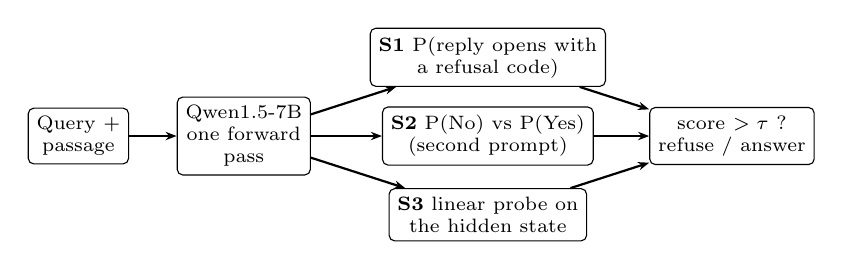
\begin{tikzpicture}[box/.style={draw,rounded corners=2pt,align=center,font=\scriptsize,inner sep=3pt},
  arr/.style={-{Stealth[length=4pt]},thick}]
\node[box] (in) at (0,0) {Query +\\passage};
\node[box] (m) at (2.1,0) {Qwen1.5-7B\\one forward\\pass};
\node[box] (s1) at (5.2,1.0) {\textbf{S1} P(reply opens with\\a refusal code)};
\node[box] (s2) at (5.2,0) {\textbf{S2} P(No) vs P(Yes)\\(second prompt)};
\node[box] (s3) at (5.2,-1.0) {\textbf{S3} linear probe on\\the hidden state};
\node[box] (d) at (8.3,0) {score $>\tau$ ?\\refuse / answer};
\draw[arr] (in) -- (m);
\foreach \n in {s1,s2,s3}{\draw[arr] (m) -- (\n); \draw[arr] (\n) -- (d);}
\end{tikzpicture}}
\caption{Extension 2: no text is generated. Each score comes from a single forward pass under its own prompt; a threshold $\tau$ (or the probe) turns each into an answer-or-refuse decision, with $\tau$ chosen on other source questions.}
\label{fig:overview}
\end{figure}

\textbf{S1: refusal-code probability.} With the original prompt, we compute the probability that the reply \emph{opens} with a refusal code. A code spans several tokens and the model sometimes wraps it, so for each wrapper $w\in\{\text{none},\ \mathtt{**},\ \mathtt{`},\ \mathtt{ANSWER:},\ \mathtt{Answer:}\}$ we take the longest token prefix $v_w$ shared by all seven codes and compute its probability by teacher forcing; the opening forms are mutually exclusive, so
\begin{equation}
p_{\text{ref}}(x)=\sum_{w}\prod_{t=1}^{|v_w|}P\!\left(v_{w,t}\mid x,v_{w,<t}\right),\quad s_1=\log\frac{p_{\text{ref}}}{1-p_{\text{ref}}}.
\end{equation}
We use $p_{\text{ref}}=0.5$ ($s_1=0$) as the natural untuned threshold; it does not reproduce the sampled baseline policy exactly, which also produces free-text refusals. The wrapped forms account for about 30\% of the baseline's coded refusals. The cached scoring was checked against a cache-free reference on a tiny random model (maximum difference $10^{-6}$).

\textbf{S2: sufficiency probability.} A second prompt asks whether the query can be answered completely and faithfully from the passage, ``Yes or No''; $s_2=\log P(\text{No})-\log P(\text{Yes})$ over the first token (mean probability mass on the two words: 1.0).

\textbf{S3: hidden-state probe.} A logistic regression on the last-token hidden state (final and middle layer, under either prompt), after standardization and PCA to 128 dimensions. It is \emph{supervised} with the benchmark's labels, unlike the baseline, so we treat it as a diagnostic of what the hidden state encodes, not as an equal-training-condition replacement for the baseline.

\textbf{Protocol.} All 100 source questions occur in any random half of the data, so tuning on one half and testing on the other would leak source questions. We instead cross-fit over source questions (5 folds): an example's own source question is never in the data used to choose its threshold (maximizing BA) or to fit its probe, whose layer and regularization are chosen by an inner grouped cross-validation. Held-out decisions are pooled for evaluation. The success rule was fixed before the run: the signal check requires the lower end of S1's AUROC interval to exceed 0.5, and the gate check requires the tuned-minus-default BA interval to lie above 0. For comparisons with the judged baseline, a rule is BETTER if the paired 95\% interval of its BA difference lies entirely above zero, WORSE if entirely below zero, and has NO CLEAR DIFFERENCE otherwise. Intervals resample source questions of the pooled held-out predictions; fitting is not repeated inside each resample, so they reflect sampling of the evaluation examples, not variability of the fitted thresholds or probe. A unit test confirms that a fold's threshold does not change when that fold's own labels are corrupted. Scoring takes about 0.3 s per example and prompt on a T4 (about 8 minutes per pass over the 1{,}600 examples), needs no judge and no API key, and costs nothing on the free tier.

\subsection{Does the signal exist?}
Table~\ref{tab:n2} shows that all three scorers separate refusal-required from answerable examples above chance on all 1{,}600 examples (lower interval bounds 0.70 and above). The probe is best; S2 is slightly better than S1 (S1 minus S2: $-0.025$, 95\% CI $[-0.047,-0.003]$), and the probe beats S1 by $+0.071$ $[+0.041,+0.102]$. Figure~\ref{fig:dist} shows the S1 score for the two groups: they overlap but are clearly shifted. The probe chose a middle-layer state in four of the five folds (three under the baseline prompt, one under the yes/no prompt) and the final-layer state of the yes/no prompt in the fifth. Tuning a threshold on S1 moves the operating point (MRR 0.59 to 0.41, FRR 0.10 to 0.26) but does not significantly improve balanced accuracy over the default (+0.015, $[-0.008,+0.036]$): it slides along one trade-off curve. The probe is better than the tuned S1 gate by $+0.053$ $[+0.024,+0.081]$.

\begin{table}[t]
\centering
\caption{Extension 2 on all 1{,}600 examples; thresholds and probe cross-fitted over source questions; 95\% cluster-bootstrap intervals.}
\label{tab:n2}
\footnotesize
\setlength{\tabcolsep}{3pt}
\begin{tabular}{lccccc}
\toprule
Scorer / rule & AUROC [95\% CI] & FRR & MRR & BA & F1 \\
\midrule
S1 refusal prob. & .726 [.699, .752] & & & & \\
\quad default ($p>0.5$) & & .103 & .590 & .654 & .561 \\
\quad tuned threshold & & .256 & .408 & .668 & .688 \\
S2 yes/no prob. & .751 [.723, .777] & & & & \\
\quad default (No $>$ Yes) & & .125 & .540 & .667 & .604 \\
\quad tuned threshold & & .321 & .329 & .675 & .732 \\
S3 hidden-state probe & .797 [.770, .825] & .250 & .307 & \textbf{.721} & .762 \\
\bottomrule
\end{tabular}
\end{table}

\begin{figure}[t]
\centering
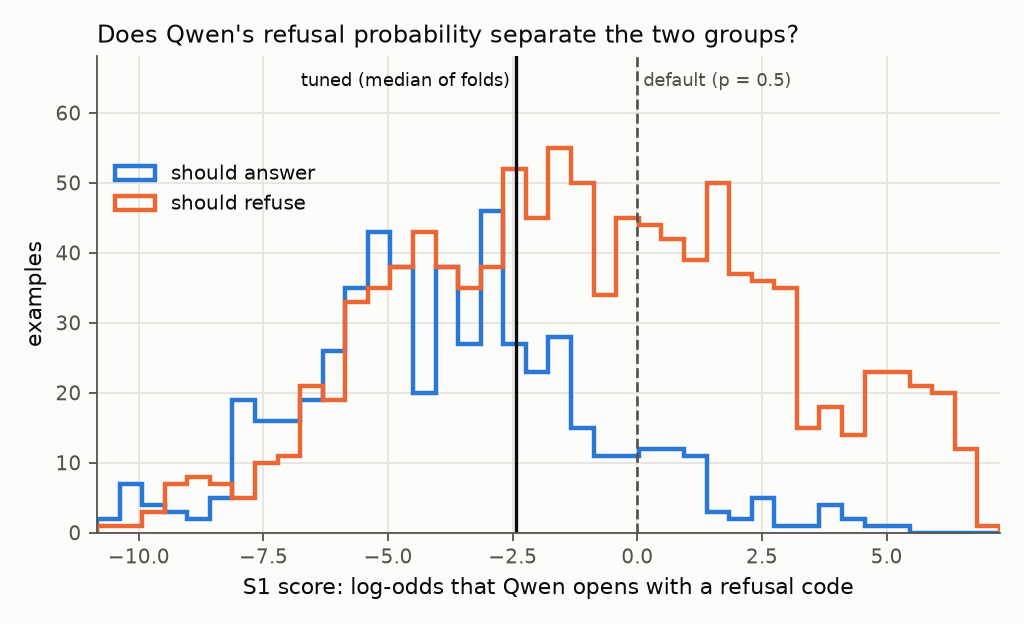
\includegraphics[width=\columnwidth]{figures/s1_distribution.png}
\caption{S1 score (log-odds that the reply opens with a refusal code) for answerable and refusal-required examples, all 1{,}600 examples. The default threshold is $s_1=0$.}
\label{fig:dist}
\end{figure}

\subsection{Is it better than the baseline?}
The fair comparison scores the judged baseline replies and the new decision rules on the same examples (Table~\ref{tab:cmp}, Fig.~\ref{fig:cmp}). A baseline reply counts as a refusal when the judge classifies it as any refusal code. Because 64\% of baseline replies are free text and depend on the Gemini judge, whereas the new rules are scored directly against the benchmark's labels, differences of a few BA points are provisional until judge agreement is validated. On the 770 graded examples the baseline reaches BA 0.688 (95\% CI $[0.654,0.722]$), higher than the 0.64 obtained by counting only clean codes, which illustrates how much a code-only reading understates it. The label-free default thresholds do not beat it, and S1's default is slightly worse ($-0.029$, $[-0.056,-0.002]$); with five comparisons and no multiplicity correction this nominal result is not robust. The tuned thresholds and S2 are indistinguishable from it. The probe is the only candidate: BA 0.718, a difference of $+0.030$ with an interval that includes zero, $[-0.012,+0.067]$. S3 uses the benchmark's labels during training and the baseline does not, so this is not a comparison under equal training conditions. It misses fewer refusals (MRR 0.29 versus 0.46) at the price of more false refusals (0.28 versus 0.17). Figure~\ref{fig:cmp} shows the baseline's operating point close to the S1 and S2 trade-off curves and just above the probe's, consistent with limited room for improvement from a global threshold alone; this is a visual observation, not a statistical test. \todo{re-run with all 1{,}560 baseline replies graded and update Table~\ref{tab:cmp}, Fig.~\ref{fig:cmp} and this paragraph}

\begin{table}[t]
\centering
\caption{Judged baseline versus the new decision rules on the same 770 examples (BA difference is rule minus baseline, 95\% cluster-bootstrap CI). Labels: whether the rule was fitted on benchmark labels.}
\label{tab:cmp}
\footnotesize
\setlength{\tabcolsep}{2.5pt}
\begin{tabular}{lcccl}
\toprule
Rule & BA & $\Delta$BA [95\% CI] & Labels & Verdict \\
\midrule
Baseline (judged) & .688 & -- & no & -- \\
S1 default & .658 & $-.029$ [$-.056$, $-.002$] & no & worse \\
S1 tuned & .671 & $-.016$ [$-.045$, $+.011$] & yes & unclear \\
S2 default & .669 & $-.018$ [$-.045$, $+.008$] & no & unclear \\
S2 tuned & .668 & $-.019$ [$-.054$, $+.016$] & yes & unclear \\
S3 probe & .718 & $+.030$ [$-.012$, $+.067$] & yes & unclear \\
\bottomrule
\end{tabular}
\end{table}

\begin{figure}[t]
\centering
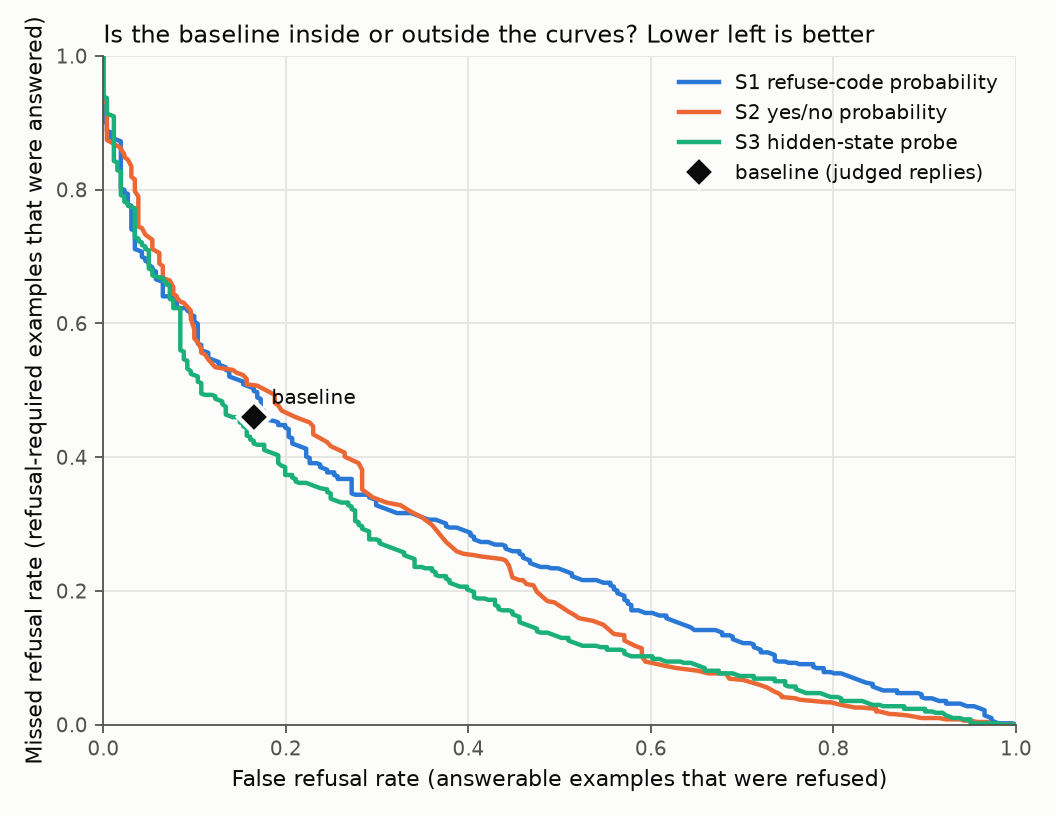
\includegraphics[width=\columnwidth]{figures/baseline_vs_scorers.png}
\caption{False versus missed refusal for every threshold of S1, S2 and S3 (lower left is better), with the judged baseline (diamond) on the same 770 examples.}
\label{fig:cmp}
\end{figure}

\subsection{Where does each rule help?}
Table~\ref{tab:type} breaks the decisions down by perturbation class, with every rule scored on the same 770 examples. The three readouts behave differently. S1 shares the baseline's profile: it still misses 66\% of ambiguity and 63\% of contradiction refusals. S2 and the probe cut contradiction misses from 0.71 (baseline) to 0.23 and 0.19, and ambiguity misses from 0.74 to 0.55 and 0.45, but pay with more false refusals on answerable examples of those classes (contradiction 0.17 to 0.50 and 0.29). The probe is the only rule that lowers the false-premise false-refusal rate below the baseline's (0.23 against 0.33; S1 and S2: 0.50 and 0.47), but it misses more false-premise refusals (0.25 against 0.19) and over-refuses granularity-mismatch examples (0.35 against 0.10). The overall BA of the probe therefore hides large class-dependent trade-offs. With 40 to 93 examples per cell, these class-level numbers are descriptive.

\begin{table}[t]
\centering
\caption{Missed / false refusal rate by perturbation class, all rules on the same 770 graded examples (thresholds as in Table~\ref{tab:n2}). Lower is better in both entries.}
\label{tab:type}
\footnotesize
\setlength{\tabcolsep}{3pt}
\begin{tabular}{lcccc}
\toprule
Class & Baseline & S1 tuned & S2 tuned & S3 probe \\
\midrule
Ambiguity & .74/.09 & .66/.11 & .55/.21 & .45/.23 \\
Contradiction & .71/.17 & .63/.24 & .23/.50 & .19/.29 \\
Missing information & .56/.22 & .51/.39 & .49/.34 & .53/.37 \\
Epistemic mismatch & .30/.12 & .19/.14 & .30/.19 & .12/.19 \\
False premise & .19/.33 & .20/.50 & .16/.47 & .25/.23 \\
Granularity mismatch & .25/.10 & .19/.23 & .25/.33 & .19/.35 \\
\bottomrule
\end{tabular}
\end{table}

\section{Discussion}
\textbf{Asking fails, reading works somewhat.} Prompting a 7B model to reason about the evidence before acting produced its worst behavior, while the same model's probabilities and hidden states separate the two groups with AUROC up to 0.80. Refusal-required status is therefore more separable in the model's scores and hidden states than in its generated decisions. We do not establish why this gap occurs, and we did not test why the model anchors on ``clear'', so we make no mechanistic claim.

\textbf{Where it works and where it does not.} On refusal-required examples, MRR is relatively low for epistemic mismatch, false premise and granularity mismatch (0.12--0.30 across rules), although several rules incur a high FRR on the corresponding answerable examples. Ambiguity, contradiction and missing information are the hard classes: S1 and the baseline miss about half or more of them, whereas S2 and the probe recover many contradictions and ambiguities, but only by refusing more answerable examples. The false-premise class is over-refused by S1 and S2 (FRR 0.50 and 0.47). Because the best threshold differs by class, a single global threshold is a blunt instrument; whether class-aware thresholds would help is an open question we did not test, and with one seed and 100 source questions the per-class numbers are descriptive, not tested.

\textbf{What this suggests.} Reading a refusal probability through a threshold is not an improvement over letting the model answer; a supervised probe shows a small positive point estimate but no clear improvement. Our result is compatible with the view that selective refusal in small models is limited by how refusal-relevant information is expressed rather than by its absence from the model's states, but it does not establish it.

\section{Limitations}
\label{sec:limits}
(i) One model, one benchmark, one seed, 4-bit weights, sampling at temperature 1.0. (ii) The judge is Gemini, not the original Claude, and has not yet been validated by our planned 30-reply hand check. Because most baseline replies depend on the judge while the new rules do not, this is the most important threat to the comparison in Table~\ref{tab:cmp}. (iii) The baseline comparison currently uses half of the graded replies, and the 40 failed examples are excluded. (iv) The probe is supervised and trained on the same 100 source questions' distribution; cross-fitting prevents source overlap but not distribution shift. (v) S1 reads only openings that start with a refusal code, so free-text refusals look like answers to it. (vi) We measure detection, not the reason for refusing and not answer correctness for the new rules. (vii) We compare five rules with 95\% intervals and no multiplicity correction, so the one ``worse'' verdict (S1 default, upper bound $-0.002$) is not robust to such a correction.

\section{Conclusion}
We reproduced the RefusalBench-NQ baseline for Qwen1.5-7B-Chat on free resources, showed that making the model diagnose the evidence before answering backfires, and showed that refusal-required status is readable from its internal signal (AUROC 0.73--0.80) yet only weakly exploitable: thresholding it does not beat the baseline and a supervised probe is at best slightly better. Future work should complete the judged baseline comparison, validate the judge, repeat the study on more models and seeds, and test readouts that target the hard classes, ambiguity and contradiction. The code, configurations and per-example scores are at \url{https://github.com/aidepartmentrah-pixel/refusalbench-reproduction}.

\bibliographystyle{IEEEtran}
\bibliography{references}

\end{document}
